\documentclass[a4paper]{article}

\usepackage[english]{babel}
\usepackage[utf8]{inputenc}
\usepackage{float}
\usepackage{amsmath}
\usepackage{graphicx}
\usepackage{subfigure}
\usepackage{natbib}
\usepackage[colorinlistoftodos]{todonotes}

\title{\bfseries{COMP90016 -- Assignment 2 }}
\author{Haonan Li}

\date{\today}

\begin{document}
\maketitle

\section{Introduction}
\label{sec:introduction}

This assignment consists of three tasks. 

In the first task, we discuss the application of HMMs to CNV detection in theory. The second task is an implementation of a CNV detection algorithm using segmentation. In the final task, we discuss the biology of a particular cancer sample.

\section{Task1}

The lectures introduced a HMM designed to detect CNVs in a haploid organism. It consisted of three states: One for the normal copy number (CP1) and two alternate copy number states (Cp0, CP2).\\

\noindent\textbf{Question 1} How would you adapt this approach to a diploid organism, such as human (with states representing different integer copy numbers)? \\

\noindent\textbf{Answer}: For a diploid organism. The normal copy number of chromosome is 2. Take account of copy number changes. four alternate copy number states should be used (CP0, CP1, CP3, CP4). All of them maybe exist in the real world. However, it should be adjust according to the datasets. If there are some bins with 5 copy numbers. We might add CP5 to the state set.\\

\noindent\textbf{Question 2}: Explain the trade-off between the sensitivity of such a HMM and the computational complexity to solve the Viterbi algorithm for it.\\

\noindent\textbf{Answer}: The complexicity of HMM model is $O(nm^2)$. Where n represents the length of the sequence and m is the number of states. If m is large, of course the experiment can contain more possible copy numbers and the result will more precisely. But it will also take more time It will take more than twice as much time for m change from 4 to 6. So, if there are almost no bin with 5 or 6 copy numbers. It is not worth to extend more states.\\

\noindent\textbf{Question 3}: Consider the data shown in Figure 1. The plot shows read depth of bins normalized by the average in a diploid organism. How would you use this data to parametrize the emission probabilities of your HMM? Explain what about Figure 1 is general and what is specific to the data that this plot was derived from. How does this affect the HMM in terms of its application to different data sets? Also, how could this data be utilized to derive the transition probabilities for a CNV detection HMM?\\

\noindent\textbf{Answer}: First, to build a HMM model, we should know each bin's copy number and average depth. We can calculate the emission probabilites by statistic of these informations. For a specified copy number CPX (X = 0,1,2,...). We count how many bins with CPX, assumed N (N>=0). And for each average read depth D (maybe a range), we count the number of bins with the read depth, assumed M. So the emission probability of CPX to read depth D is M/N. 

In Figure 1. There is a peak whose ratio is 1 which is general for diploid organism. But another peak with ratio=0.5 is spicific, which means this sample have some bins with deletions. This will increase the predictions of deletion if apply this to other data sets. 

Computing transation probabilities is similar with computing emission probalabilitits. Count the changes copy number pairs of adjacent bins. And compute the proportion of the end state from a specified start state.\\

\noindent\textbf{Question 4}: Describe why a HMM, such as discussed in this task is not very useful for non-clonal data (such as shown in Figure 2 below). Could this shortcoming be alleviated by introducing non-integer CN states?

\noindent\textbf{Answer}:  

\section{Task 2}

The implementation of cirular binary segmentation is not complex. 

First, inputing. Read data from file and build two lists, one is to store the tuple of start and end positions, the other stores the read depths of all bins. 

Second, init the settings. We use numoy to speed up computing. Transfer the list of read depths to numpy array. Then take the median from the first third of the input read depths as `normal' bin m. Tranform read depth each bin b into log ratios $log2(b/m)$. Then remove extreme values, specifically, set any log2-ratio that are larger then 2 or smaller than -5 to 0. After this init a segment mark array with 0 for later recersive use. 

Third, a revursive cbs function, this is the most important part of the algorithm. The function have five input parameters: log-ratio array $X$, segment mark array $I$, start position $a$, end position $b$ and z-threshold $t$. For each call of the function. First cut X from a to b, which is the current interval we analyze, name it $X'$. 

Then compute cumulative sum of bins $S_i = X_1+X_2+...+X_i$

After computing cumulative sum. We build a 2d array $Z$ and compute $Z$ by:

\begin{equation*}
Z_{ij}=(\frac{1}{j-i}+\frac{1}{n-j+i})^{-\frac{1}{2}}\times (\frac{S_j-S_i}{j-i}-\frac{S_n-S_j+S_i}{n-j+i})
\end{equation*}

Then find the maximum of $Z$, if the maximum is larger than threshold $t$, its coordinates are new segment points, suppose $x,y$. We mark them in segment mark array I (set corresponding positions to 1) and call three new cbs functions with new interval (a,x),(x,y),(y,b).

Finally, the segment mark array should have marked with 1 in some positions. Find the corresponding interval between two adjacent marks. Compute the average log-ratio and output.

As for the theoretical complexity of the algorithm. For a file with n bins. we compute a $n\times n$ matrix and seperate it to 3 segment and compute recursively. So the complexity is:

\begin{equation*}
Complexity = O(n^2 + 3^{1}(\frac{n}{3^{1}})^2 + 3^{2}(\frac{n}{3^{2}})^2+...+3^{t}(\frac{n}{3^{t}})^2)=O(n^2)
\end{equation*}

\section{Task 3}

\noindent 1. Figure \ref{fig} visulize the reported CNVs.

\begin{figure}[h]
	\centering
		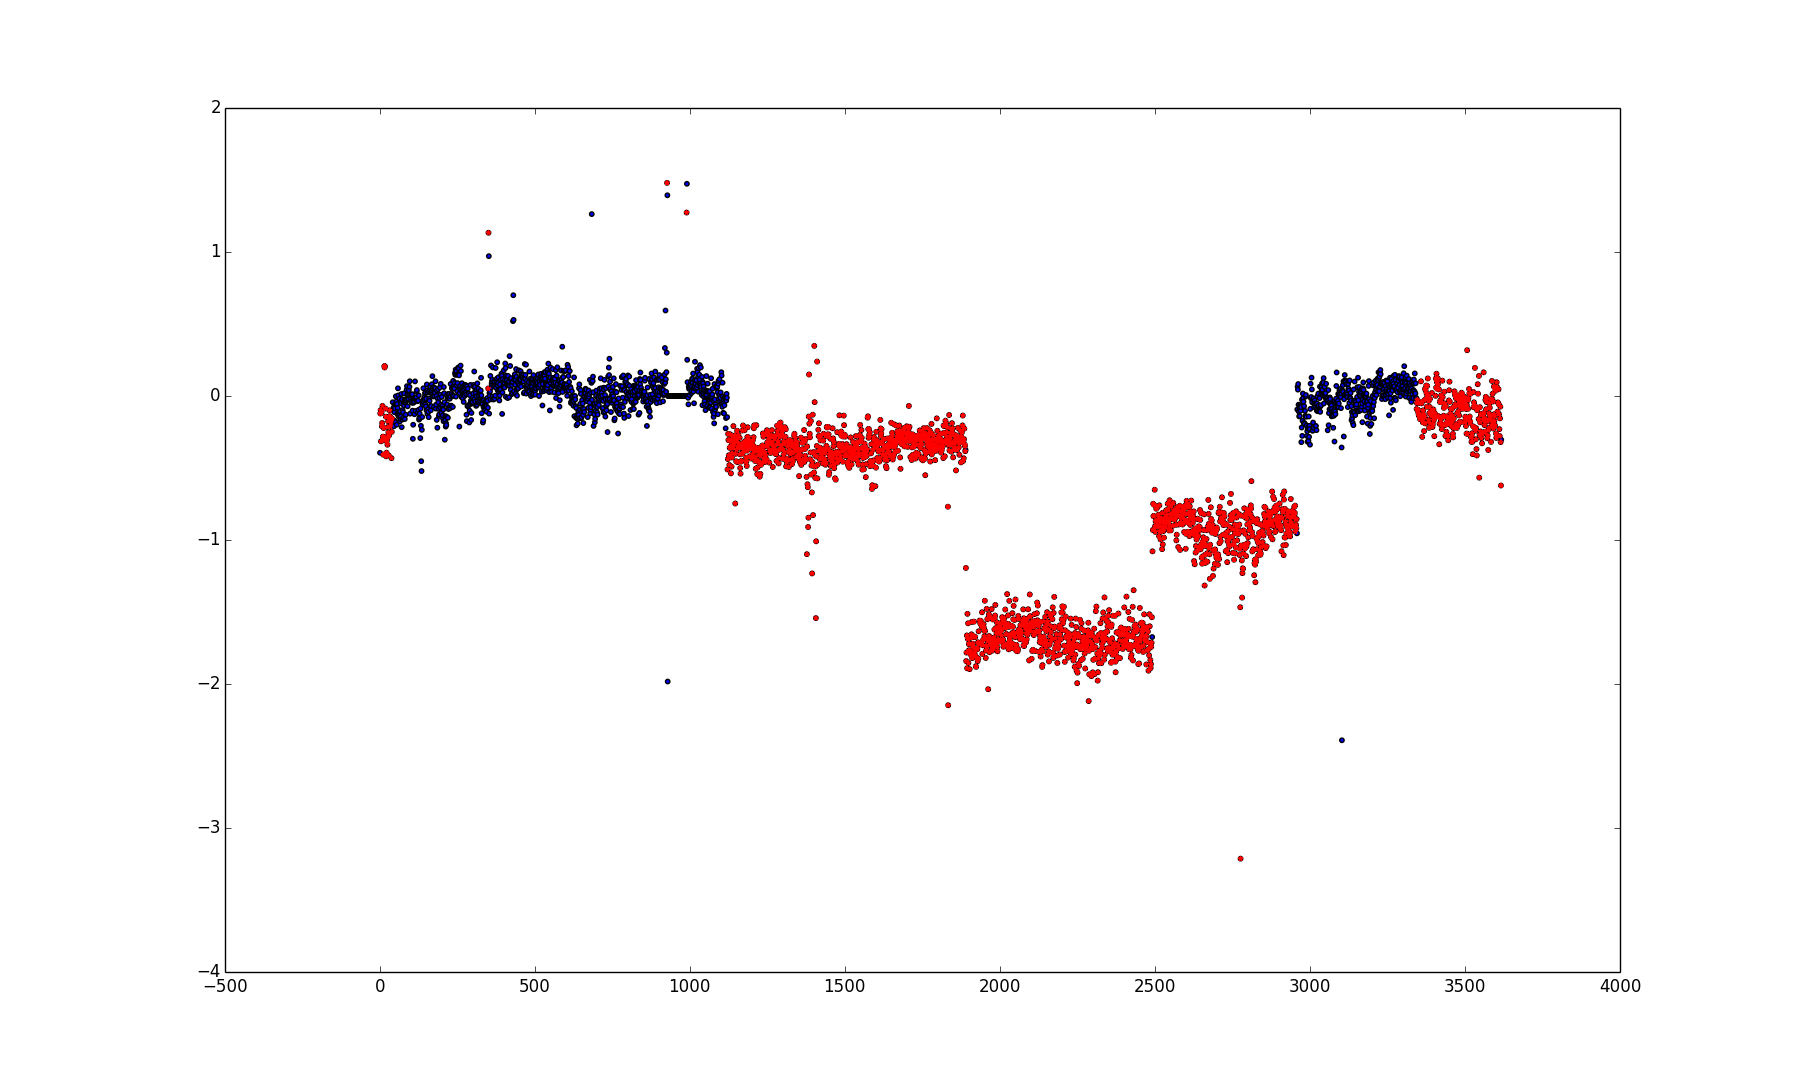
\includegraphics[width=0.8\textwidth]{snv.png}
	\caption{Visulization of CNV. (The red part is reported CNVs)}
	\label{fig} 
\end{figure}

\noindent 2. To increase sensitivity, we can decrease the Z-threshold, this will lead to more segmentations of the bins meanwhile decreasing the average range of each bins. 

\noindent 3. Biology analyze of three large CNVs in the data:

\textbf{a. 50-90Mbp}
\begin{equation*}
logR = -0.3 
\end{equation*}
\begin{equation*}
observed\ copy\ number  = 2^{1-0.3}=1.6
\end{equation*}

assume $colonality = c$, with $CN = x$, there is:

\begin{equation*}
xc+2(1-c) = 1.6
\end{equation*}

possible $(x,c)$ pairs:

\begin{equation*}
x = 1, c = 0.4
\end{equation*}
\begin{equation*}
x = 0, c = 0.2
\end{equation*}

\textbf{b. 90-125Mbp}
\begin{equation*}
logR = -1.3 
\end{equation*}
\begin{equation*}
observed\ copy\ number  = 2^{1-1.3}=0.8
\end{equation*}

assume $colonality = c$, with $CN = x$, there is:

\begin{equation*}
xc+2(1-c) = 0.8
\end{equation*}

possible $(x,c)$ pairs:

\begin{equation*}
x = 0, c = 0.6
\end{equation*}

\textbf{c. 125-140Mbp}
\begin{equation*}
logR = -0.8
\end{equation*}
\begin{equation*}
observed\ copy\ number  = 2^{1-0.3}=1.1
\end{equation*}

assume $colonality = c$, with $CN = x$, there is:

\begin{equation*}
xc+2(1-c) = 1.1
\end{equation*}

possible $(x,c)$ pairs:

\begin{equation*}
x = 1, c = 0.9
\end{equation*}
\begin{equation*}
x = 0, c = 0.45
\end{equation*}

\noindent 4. Assume three CNVs happens independentely on two clones. There are four possible cases for these three CNVs, show in Table \ref{tb:1}

\begin{table}[h]
	\centering
	\begin{tabular}{c|cccccc}
		case\# & $x_1$ & $c_1$ & $x_2$ & $c_2$ & $x_3$ & $c_3$ \\
		\hline
		1 & 0 & 0.2 & 0 & 0.6 & 0 & 0.45 \\
		2 & 0 & 0.2 & 0 & 0.6 & 1 & 0.9 \\
		3 & 1 & 0.4 & 0 & 0.6 & 0 & 0.45 \\
		4 & 1 & 0.4 & 0 & 0.6 & 1 & 0.9 \\
	\end{tabular}
	\label{tb:1}
\end{table}

For the first and third CNVs, both single and double loss of DNV are possible, for the second CNVs, double copy losses of DNA happens.

\bibliographystyle{plainnat}
\bibliography{report}

\end{document}